\documentclass{xjtureport}
% =============================================
% Part 0 Edit the info
% =============================================

\major{计算机001班}
\name{曾锦程}
\title{SDN实验报告}
\stuid{2203613040}
\college{计算机学院}
\date{\zhtoday}
\lab{}
\course{软件定义网络}
\instructor{张鹏}
\grades{}
\expname{Lab3 测量链路时延与链路容忍}
\exptype{设计实验}
\partner{}

\begin{document}
% =============================================
% Part 1 Header
% =============================================
\makecover
\makeheader
\tableofcontents
\newpage
% =============================================
% Part 2 Main document
% =============================================

\section{实验目的}
通过本次实验,希望大家掌握以下内容:\par
1.学习利用 \texttt{ryu.topology.api} 发现网络拓扑。\par
2.学习利用 \texttt{LLDP} 和 \texttt{Echo} 数据包测量链路时延。\par
3.学习计算基于跳数和基于时延的最短路由。\par
4.学习设计能够容忍链路故障的路由策略。\par
5.分析网络集中式控制与分布式控制的差异,思考SDN的得与失。
\section{问题背景}
\begin{figure}[H]
	\centering
	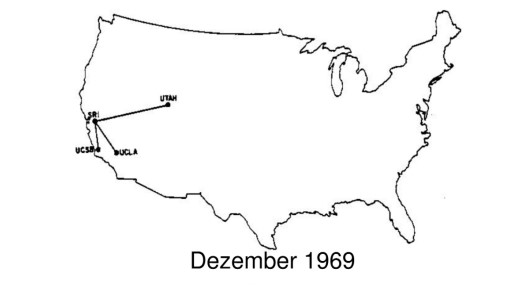
\includegraphics[width=0.9\linewidth]{1.jpg}
	\caption{TOPO-1970}
\end{figure}
时间来到1970年,在你的建设下 \texttt{ARPANET} 飞速发展,在一年内从原来西部4个结点组成的简单网络逐渐
发展为拥有9个结点,横跨东西海岸,初具规模的网络。\par
\texttt{ARPANET} 的拓展极大地便利了东西海岸之间的通信,但用户仍然十分关心网络服务的性能。一条时延较
小的转发路由将显著提升用户体验,尤其是在一些实时性要求很高的应用场景下。另外,路由策略对网
络故障的容忍能力也是影响用户体验的重要因素,好的路由策略能够向用户隐藏一定程度的链路故障,
使得个别链路断开后用户间的通信不至于中断。\par
\texttt{SDN} 是一种集中式控制的网络架构,控制器可以方便地获取网络拓扑、各链路和交换机的性能指标、网
络故障和拓扑变化等全局信息,这也是 \texttt{SDN} 的优势之一。在掌握全局信息的基础上, \texttt{SDN} 就能实现更高
效、更健壮的路由策略。\par
在正式任务之前,为帮助同学们理解,本指导书直接给出了一个示例。请运行示例程序,理解怎样利用
\texttt{ryu.topology.api} 获取网络拓扑,并计算跳数最少的路由。\par
跳数最少的路由不一定是最快的路由,在实验任务一中,你将学习怎样利用 \texttt{LLDP} 和 \texttt{Echo} 数据包测量链
路时延,并计算时延最小的路由。\par
1970年的网络硬件发展尚不成熟,通信链路和交换机端口发生故障的概率较高。在实验任务二中,你将
学习在链路不可靠的情况下,设计对链路故障有一定容忍能力的路由策略。
\section{基本实验理论}
\subsection{拓扑感知}
控制器首先要获取网络的拓扑结构,才能够对网络进行各种测量分析,网络拓扑主要包括主机、链路和
交换机的相关信息。
\subsection{链路发现原理}
LLDP(Link Layer Discover Protocol) 即链路层发现协议, Ryu 主要利用 LLDP 发现网络拓扑。
LLDP 被封装在以太网帧中,结构如下图。其中深灰色的即为 LLDP 负载, Chassis ID TLV , Port ID
TLV 和 Time to live TLV 是三个强制字段,分别代表交换机标识符(在局域网中是独一无二的),端
口号和 TTL 。
\begin{figure}[H]
	\centering
	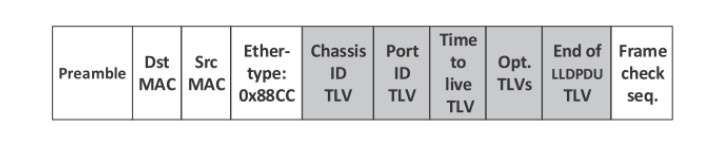
\includegraphics[width=0.9\linewidth]{2.jpg}
	\caption{LLDP报文格式}
\end{figure}
接下来介绍 Ryu 如何利用 LLDP 发现链路,假设有两个 OpenFlow 交换机连接在控制器上,如下图:
\begin{figure}[H]
	\centering
	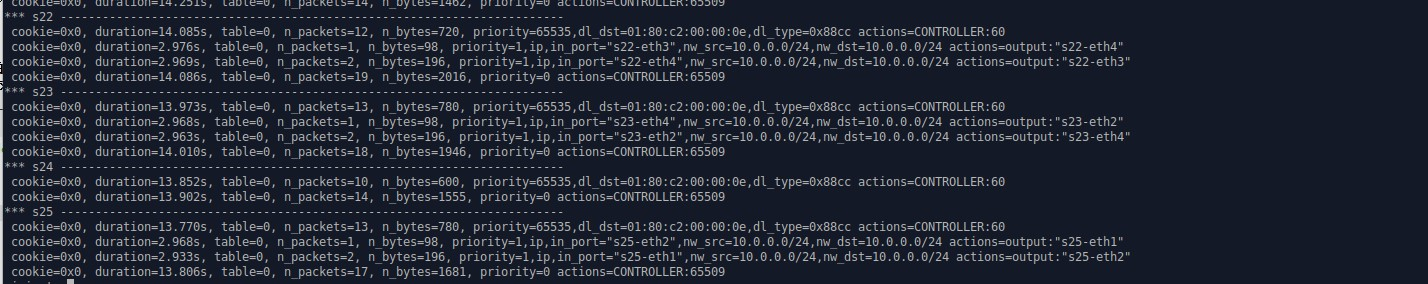
\includegraphics[width=0.9\linewidth]{3.jpg}
	\caption{LLDP原理图}
\end{figure}
1. SDN 控制器构造 PacketOut 消息向 S1 的三个端口分别发送 LLDP 数据包,其中将 Chassis ID
TLV 和 Port ID TLV 分别置为 S1 的 dpid 和端口号;\par
2. 控制器向交换机 S1 中下发流表,流表规则为:将从 Controller 端口收到的 LLDP 数据包从他的对
应端口发送出去;\par
3. 控制器向交换机 S2 中下发流表,流表规则为:将从非 Controller 接收到的 LLDP 数据包发送给控
制器;\par
4. 控制器通过解析 LLDP 数据包,得到链路的源交换机,源接口,通过收到的 PacketIn 消息知道目
的交换机和目的接口。
\subsection{沉默主机现象}
主机如果没有主动发送过数据包,控制器就无法发现主机。运行前面的 NetworkAwareness.py 时,你
可能会看到 host 输出为空,这就是沉默主机现象导致的。你可以在 mininet 中运行 pingall 指令,令
每个主机发出 ICMP 数据包,这样控制器就能够发现主机。当然命令的结果是 ping 不通,因为程序中并
没有下发路由的代码。
\subsection{链路时延计算}
测量链路时延的思路可参考下图:
\begin{figure}[H]
	\centering
	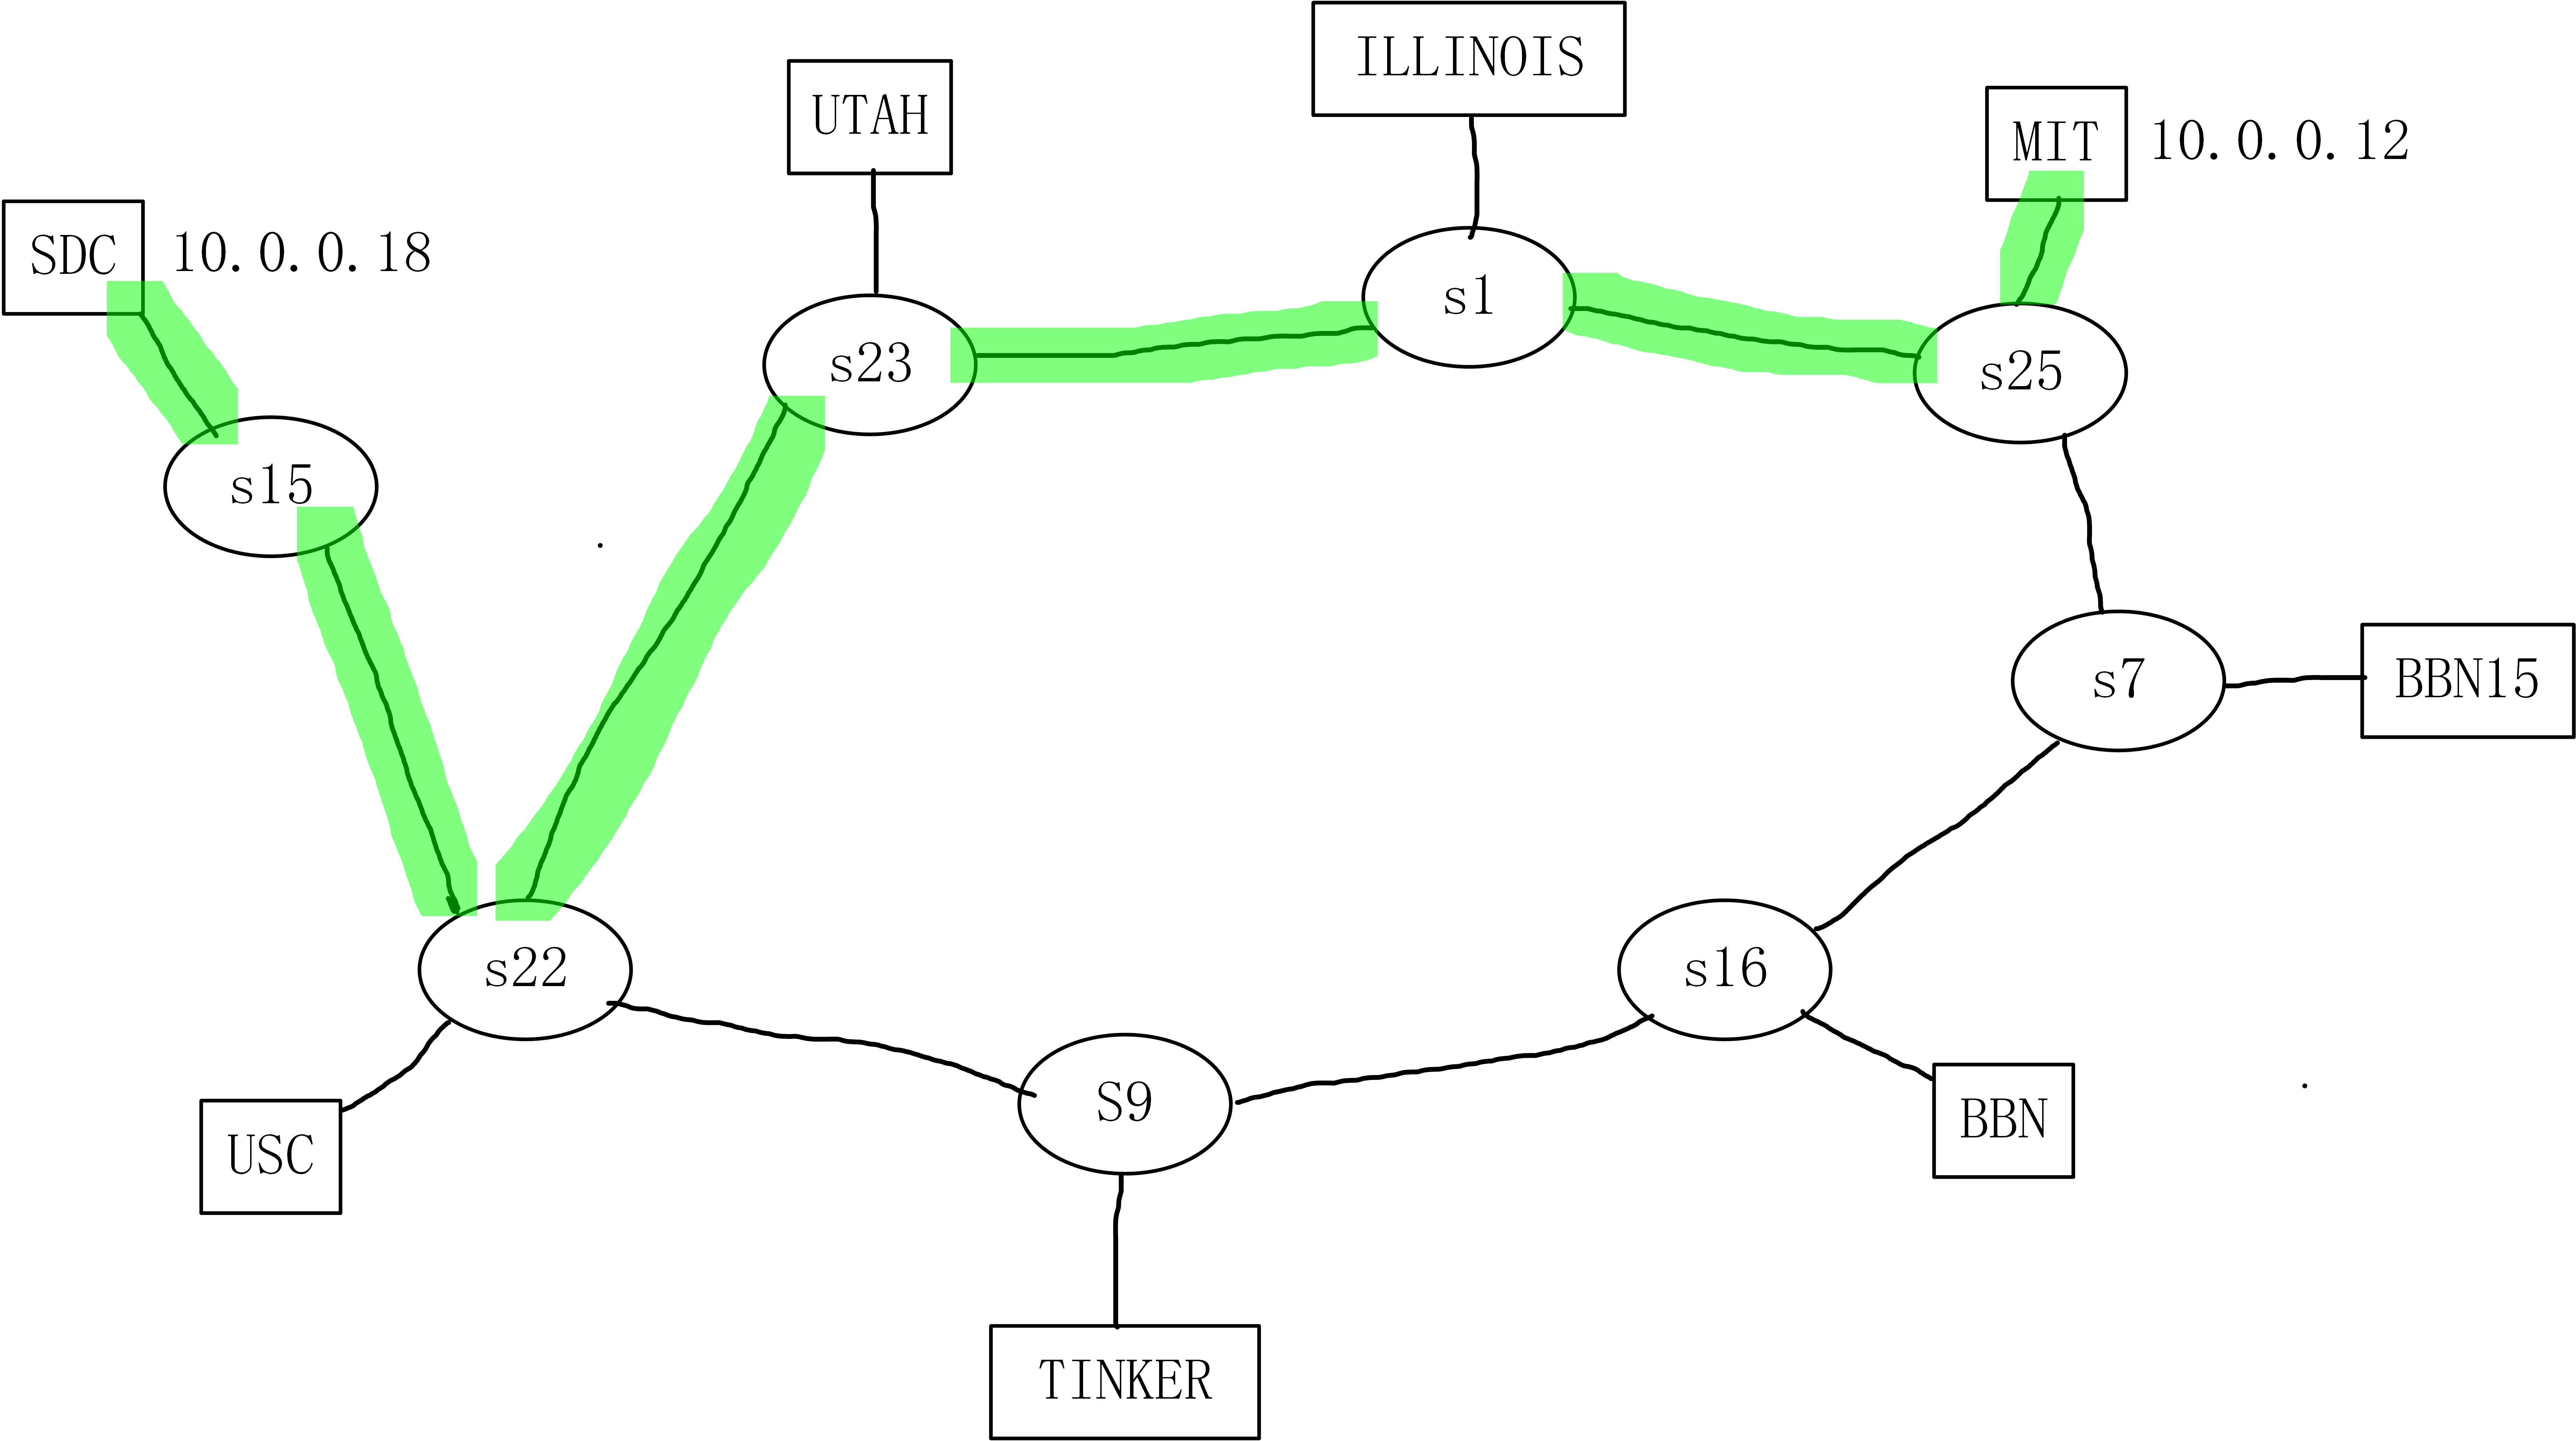
\includegraphics[width=0.9\linewidth]{4.jpg}
	\caption{计算链路时延}
\end{figure}
控制器将带有时间戳的 LLDP 报文下发给 S1 , S1 转发给 S2 , S2 上传回控制器(即内圈红色箭头的路
径),根据收到的时间和发送时间即可计算出\textbf{控制器经 S1 到 S2 再返回控制器的时延},记为
lldp\_delay\_s12\par
反之,\textbf{控制器经 S2 到 S1 再返回控制器的时延},记为 lldp\_delay\_s21\par
交换机收到控制器发来的Echo报文后会立即回复控制器,我们可以利用 Echo Request/Reply 报文求出
\textbf{控制器到 S1 、 S2 的往返时延},记为 echo\_delay\_s1 , echo\_delay\_s2\par
则 S1 到 S2 的时延:
$$
 delay = (lldp\_delay\_s_{12} + lldp\_delay\_s_{21} - echo\_delay\_s_{1} -
echo\_delay\_s_{2}) / 2
$$
\section{必做题:链路时延测量}
\subsection{测量LLDP Delay}
这里需要修改RYU的源码并编译,指导手册中有具体步骤,这里不再赘述。下面是代码中对LLDP Delay的测量:
\begin{lstlisting}[language=python]
	# __init__() -----------networkawareness.py
	self.lldp_delay = {}
	
	# lldp delay -----------networkawareness.py
	@set_ev_cls(ofp_event.EventOFPPacketIn, MAIN_DISPATCHER)
	def packet_in_handler(self, ev):
		msg = ev.msg
		dp = msg.datapath
		ofp = dp.ofproto
		parser = dp.ofproto_parser
		dpid = dp.id
	
		pkt = packet.Packet(msg.data)
		eth_pkt = pkt.get_protocol(ethernet.ethernet)
		arp_pkt = pkt.get_protocol(arp.arp)
		pkt_type = eth_pkt.ethertype
	
		if pkt_type == ether_types.ETH_TYPE_LLDP:
			src_dpid, src_port_no = LLDPPacket.lldp_parse(msg.data)
	
			if self.switches is None:
				self.switches = lookup_service_brick('switches')
	
			for port in self.switches.ports.keys():
				if src_dpid == port.dpid and src_port_no == port.port_no:
					self.lldp_delay[(src_dpid,dpid)] = self.switches.ports[port].delay * 1000
\end{lstlisting}	
\quad \quad 上述代码是调用了对RYU源码编译后的新变量,获取时延,值得注意的是这里将时延乘以1000,因为python的\texttt{time.time()}记录的单位是秒,需要转换为毫秒单位。
\subsection{测量ECHO Delay}
即让控制器给交换机发送ECHO request消息,然后再让交换机返回给控制器,通过两个时间戳来得到ECHO时间,同时这里时间差也乘以1000,保证单位一致。
\begin{lstlisting}[language=python]
	#reply and compute the ECHO Delay
	@set_ev_cls(ofp_event.EventOFPEchoReply, [MAIN_DISPATCHER,CONFIG_DISPATCHER,HANDSHAKE_DISPATCHER])
	def echo_reply_handler(self,ev):
		now_timestamp = time.time()
		try:
			echo_delay = now_timestamp - eval(ev.msg.data)
			self.controller_switch_delay[ev.msg.datapath.id]=echo_delay*1000
		except:
			return
			
	#send_echo_request
	def send_echo_request(self, switch):
		datapath=switch.dp
		parser=datapath.ofproto_parser
		echo_req=parser.OFPEchoRequest(datapath,data=bytes("%.12f"%time.time()))
		datapath.send_msg(echo_req)	
\end{lstlisting}
\subsection{计算总时延}
以下是计算总时延的代码,\texttt{\_get\_topology()}函数本身是一个不断运行的线程,所以我们在这里获取时延,来得到不断的时延更新。值得注意的是,这里计算echo\_request的过程中需要\texttt{hub.sleep(0.5)}来暂停一下,如果不暂停的话,ehco delay 非常大,不符合常理。这里猜测原因是:如果快速给每个交换机发送echo\_request,每个交换机会同时快速发送echo\_reply到控制器,而控制器没办法一下子同时处理,则需要排队拖慢ofp\_event.EventOFPEchoReply的处理速度,导致测量误差非常大。(主要是该线程是非抢占的,导致实际抓包和处理时间不一致,echo delay的时间是需要获取运行时的时间戳的,但是实际上时收到echo request的包后一段时间,才开始运行代码)
\begin{figure}[H]
	\centering
	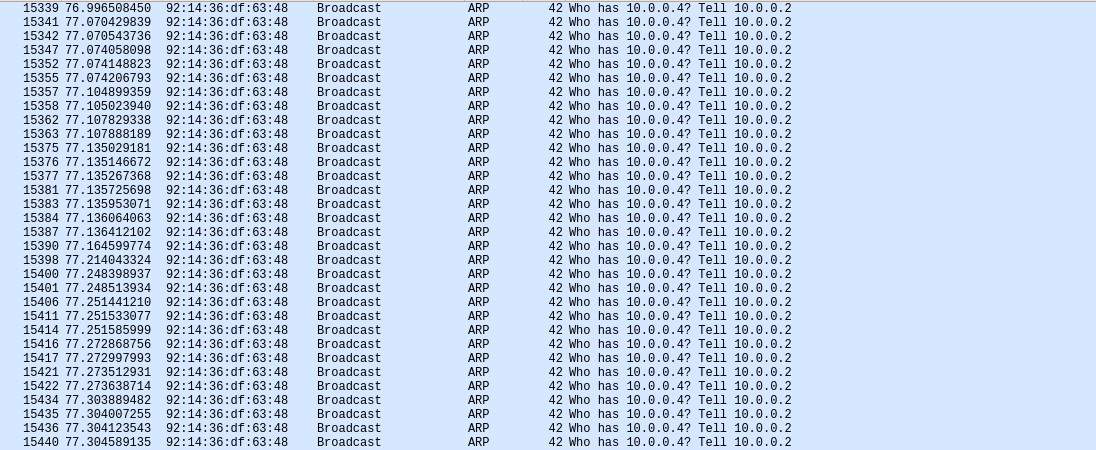
\includegraphics[width=0.9\linewidth]{7.jpg}
	\caption{错误测量echo delay(dpid:echo delay)(不准确)}
\end{figure}
\begin{figure}[H]
	\centering
	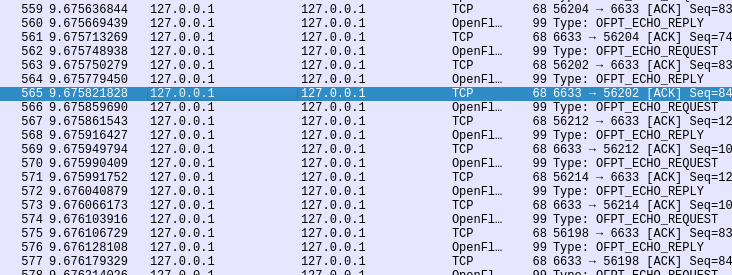
\includegraphics[width=0.7\linewidth]{6.png}
	\caption{实际echo delay(准确)}
\end{figure}
\begin{figure}[H]
	\centering
	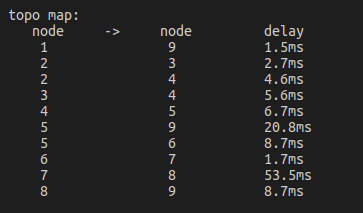
\includegraphics[width=0.6\linewidth]{7.png}
	\caption{错误链路时延}
\end{figure}
同时这里如果计算出delay<0时,让delay为0。经过多次实验,发现不存在delay<0的情况,猜测是发生了上述情况导致的。
\begin{lstlisting}[language=python]
	def _get_topology(self):
	_hosts, _switches, _links = None, None, None
	while True:
		hosts = get_host(self)
		switches = get_switch(self)
		links = get_link(self)
		
		# update topo_map when topology change
		if [str(x) for x in hosts] == _hosts and [str(x) for x in switches] == _switches and [str(x) for x in links] == _links:
			continue
		_hosts, _switches, _links = [str(x) for x in hosts], [str(x) for x in switches], [str(x) for x in links]
	
		for switch in switches:
			self.port_info.setdefault(switch.dp.id, set())
			# record all ports
			for port in switch.ports:
				self.port_info[switch.dp.id].add(port.port_no)
			self.send_echo_request(switch)
			hub.sleep(0.5)
	
		for host in hosts:
			# take one ipv4 address as host id
			if host.ipv4:
				self.link_info[(host.port.dpid, host.ipv4[0])] = host.port.port_no
				self.topo_map.add_edge(host.ipv4[0], host.port.dpid, hop=1, delay=0, is_host=True)
		for link in links:
			# delete ports linked switches
			self.port_info[link.src.dpid].discard(link.src.port_no)
			self.port_info[link.dst.dpid].discard(link.dst.port_no)
	
			# s1 -> s2: s1.port, s2 -> s1: s2.port
			self.port_link[(link.src.dpid,link.src.port_no)]=(link.src.dpid, link.dst.dpid)
			self.port_link[(link.dst.dpid,link.dst.port_no)] = (link.dst.dpid, link.src.dpid)
	
			self.link_info[(link.src.dpid, link.dst.dpid)] = link.src.port_no
			self.link_info[(link.dst.dpid, link.src.dpid)] = link.dst.port_no
	
			delay_src_to_dst = 0
			delay_dst_to_src = 0
			delay_ctl_to_src = 0
			delay_ctl_to_dst = 0
			
			if (link.src.dpid,link.dst.dpid) in self.lldp_delay:
				delay_src_to_dst = self.lldp_delay[(link.src.dpid,link.dst.dpid)]
			if (link.dst.dpid,link.src.dpid) in self.lldp_delay:
				delay_dst_to_src = self.lldp_delay[(link.dst.dpid,link.src.dpid)]
			if link.src.dpid in self.controller_switch_delay:
				delay_ctl_to_src = self.controller_switch_delay[link.src.dpid]
			if link.dst.dpid in self.controller_switch_delay:
				delay_ctl_to_dst = self.controller_switch_delay[link.dst.dpid]
			delay=(delay_src_to_dst + delay_dst_to_src - delay_ctl_to_src - delay_ctl_to_dst) / 2
			if delay < 0:
				delay = 0
			self.delay[(link.src.dpid, link.dst.dpid)] = delay
			self.topo_map.add_edge(link.src.dpid, link.dst.dpid, hop=1, delay=delay,is_host=False)
		if self.weight == 'hop':
			self.show_topo_map_1()
		if self.weight == 'delay':
			self.show_topo_map_2()
		hub.sleep(GET_TOPOLOGY_INTERVAL)
\end{lstlisting}
\subsection{测量结果}
\begin{figure}[H]
	\centering
	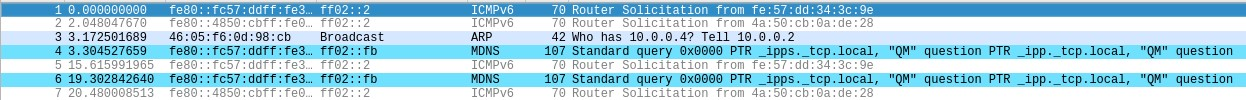
\includegraphics[width=0.9\linewidth]{8.jpg}
	\caption{测量delay结果}
\end{figure}
\begin{figure}[H]
	\centering
	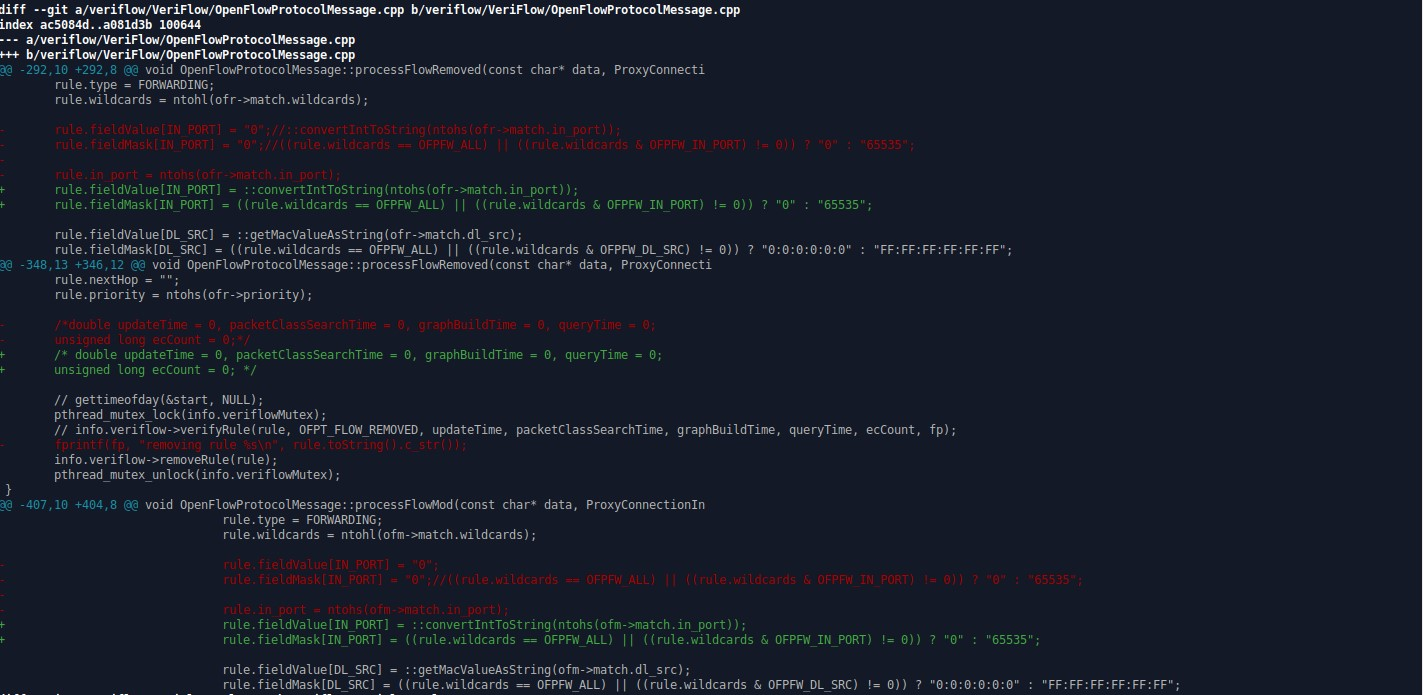
\includegraphics[width=0.9\linewidth]{9.jpg}
	\caption{理论delay结果}
\end{figure}
\begin{figure}[H]
	\centering
	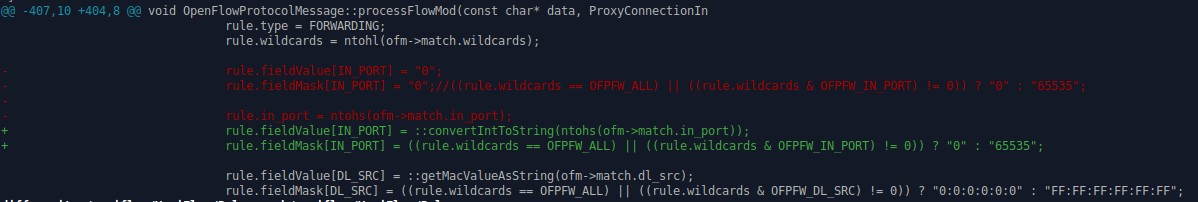
\includegraphics[width=0.9\linewidth]{10.jpg}
	\caption{将delay作为权值,来得到最短路径}
\end{figure}
可以发现测量结果较为精准,能得到好的结果。
\section{选做题:容忍链路故障}
\subsection{理论结果计算}
\begin{figure}[H]
	\centering
	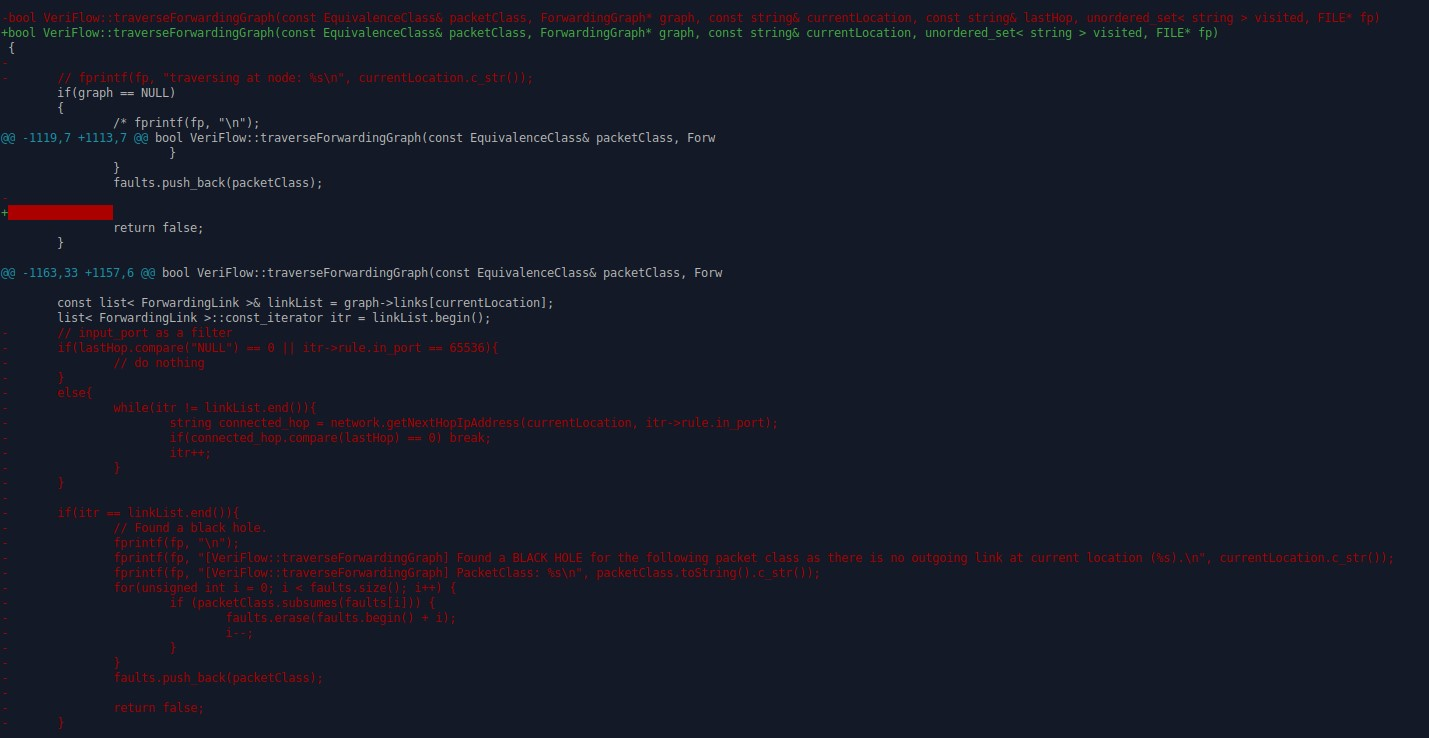
\includegraphics[width=0.9\linewidth]{11.jpg}
	\caption{实验带权图}
\end{figure}
如图为自己画的带权图,可以理论计算出SDC->MIT的最优路径为:
$$
SDC -> S6 -> S5 -> S9 -> S8 -> MIT
$$
$$
Delay=63ms
$$
$$
RTT=126ms
$$
\quad \quad 发生故障后,理论SDC->MIT路径为:
$$
SDC -> S6 -> S7 -> S8 -> MIT
$$
$$
Delay=72ms
$$
$$
RTT=144ms
$$
\subsection{关键代码}
如下代码的操作是:删除所有交换机连向的主机端口,让主机下次ping必定触发Packetin消息。下一次交换机将
匹配默认流表项,向控制器发送 packet\_in 消息,控制器重新计算并下发最小时延路径。\par
同时值得注意的是:本实验可以不用下发arp的流表来实现arp环路处理,因为本实验会专门下发srcip、dstip的流表,arp学习到的mac\_to\_port没有那么重要。
\begin{lstlisting}[language=python]
	@set_ev_cls(ofp_event.EventOFPPortStatus, MAIN_DISPATCHER)
	def port_status_handler(self, ev):
		msg=ev.msg
		datapath=msg.datapath
		ofproto=datapath.ofproto
		parser=datapath.ofproto_parser
		if msg.reason in [ofproto.OFPPR_ADD, ofproto.OFPPR_MODIFY]:
			datapath.ports[msg.desc.port_no]=msg.desc
			self.topo_map.clear()
			for dpid in self.port_info.keys():
				for port in self.port_info[dpid]:
					match=parser.OFPMatch(in_port=port)
					self.delete_flow(self.switch_info[dpid],match)
		elif msg.reason == ofproto.OFPPR_DELETE:
			datapath.ports.pop(msg.desc.port_no, None)
		else:
			return
		self.send_event_to_observers(ofp_event.EventOFPPortStateChange(datapath, msg.reason, 	msg.desc.port_no),datapath.state)
\end{lstlisting}
\subsection{实验结果}
可以看出很好地实现了结果,第一次选择RTT=126ms,符合理论值,故障后变成RTT=144ms,最后恢复变成RTT=126ms。说明了链路具有较好的容忍能力,测量结果较为精确。
\begin{figure}[H]
	\centering
	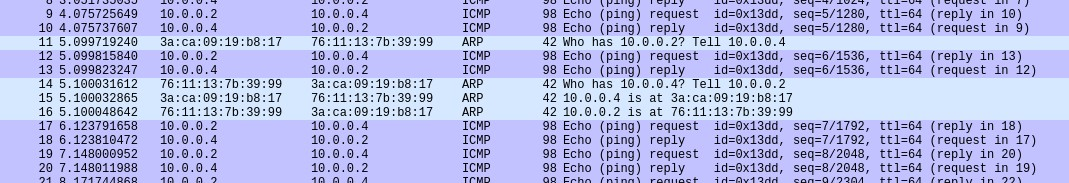
\includegraphics[width=0.9\linewidth]{12.jpg}
	\caption{第一次选择最优路径}
\end{figure}
\begin{figure}[H]
	\centering
	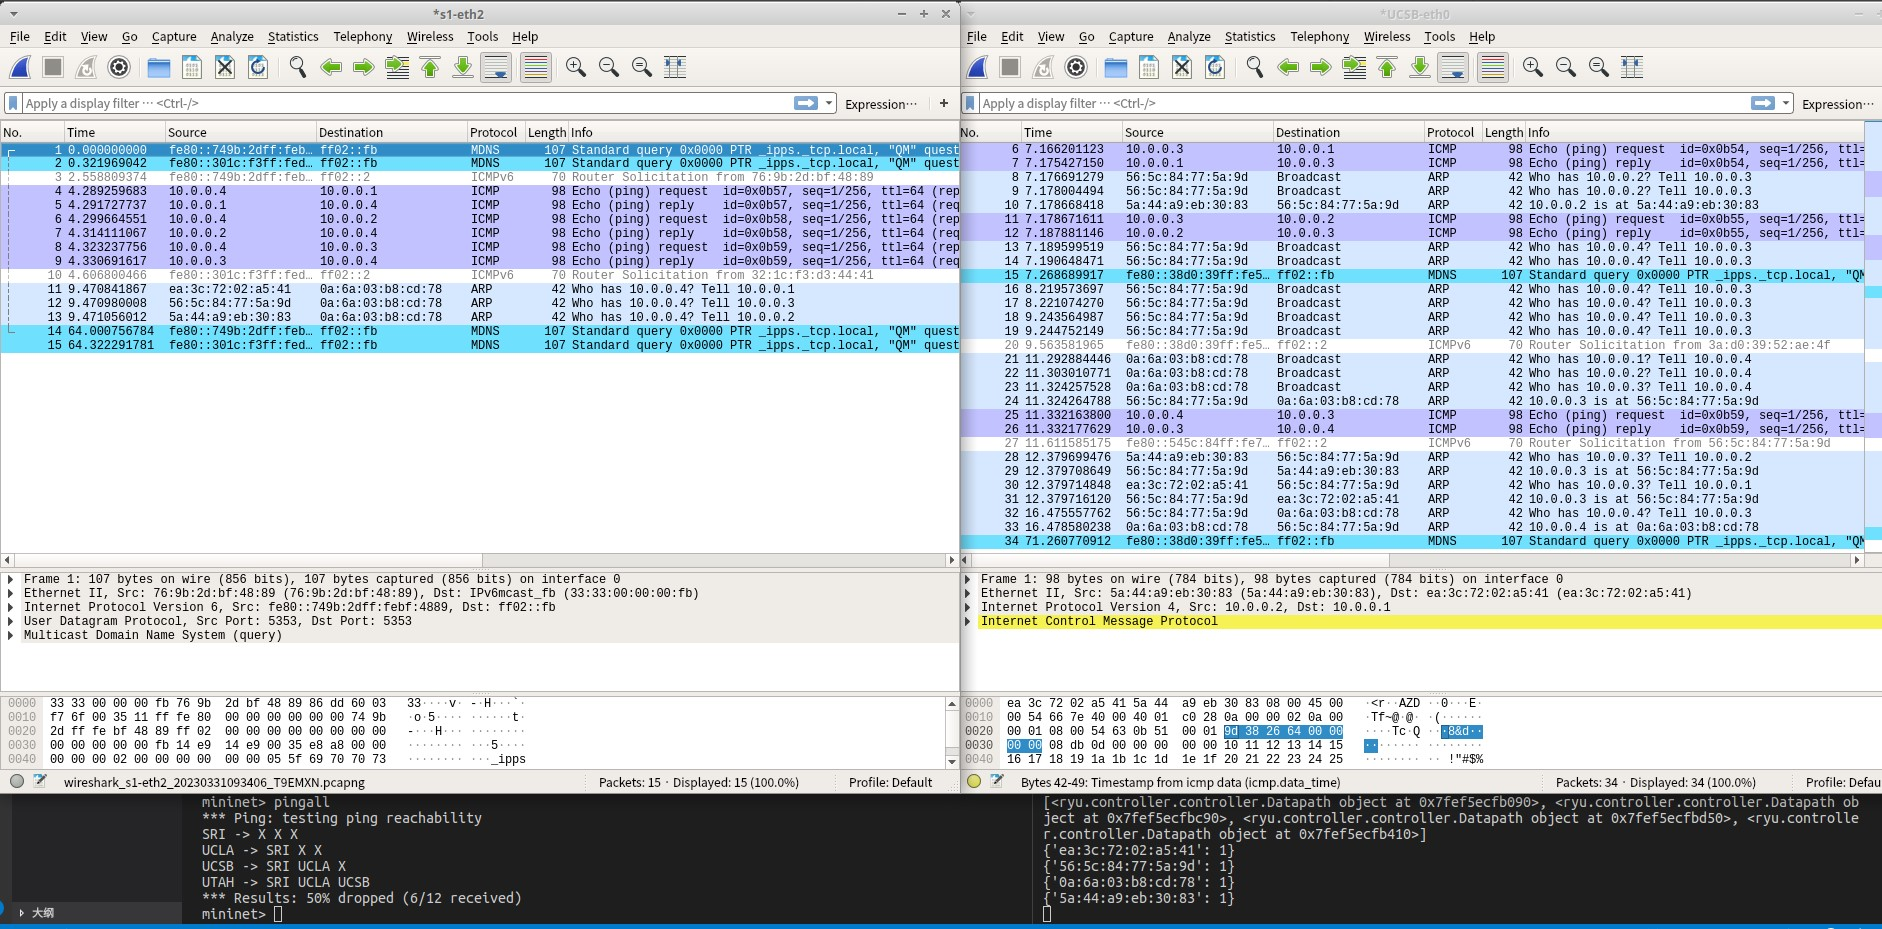
\includegraphics[width=0.9\linewidth]{13.jpg}
	\caption{故障后选择次优路径}
\end{figure}
\begin{figure}[H]
	\centering
	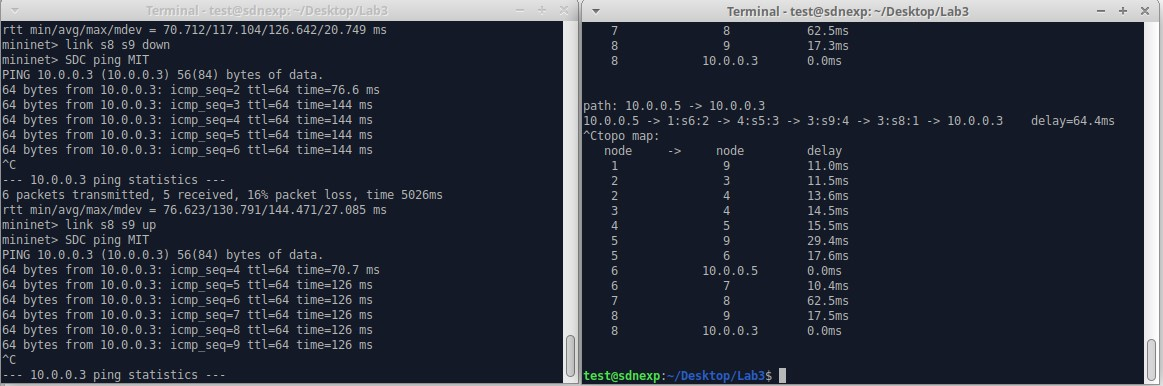
\includegraphics[width=0.9\linewidth]{14.jpg}
	\caption{恢复后选择原路径}
\end{figure}
\section{实验感悟}
1.Mininet和RYU控制器本质上还是一个虚拟的模拟器,实际处理时延等等受到操作系统、计算机的限制。\par
2.学会了通过抓包和代码结合分析问题,解决问题。\par 
3.实际实验中,ping的情况非常不稳定,经常会跳到一个更大的值,不知道是什么原因导致的,但是查找流表发现没有问题,猜测可能又是线程调度的问题。\par
\section{附录}
\subsection{networkawareness1.py}
\begin{lstlisting}[language=python]
from ryu.base import app_manager
from ryu.base.app_manager import lookup_service_brick
from ryu.ofproto import ofproto_v1_3
from ryu.controller.handler import set_ev_cls
from ryu.controller.handler import MAIN_DISPATCHER, CONFIG_DISPATCHER, DEAD_DISPATCHER, HANDSHAKE_DISPATCHER
from ryu.controller import ofp_event
from ryu.lib.packet import packet
from ryu.lib.packet import ethernet, arp
from ryu.lib.packet import ether_types
from ryu.lib import hub
from ryu.topology import event
from ryu.topology.api import get_host, get_link, get_switch
from ryu.topology.switches import LLDPPacket

import networkx as nx
import copy
import time


GET_TOPOLOGY_INTERVAL = 2
SEND_ECHO_REQUEST_INTERVAL = .05
GET_DELAY_INTERVAL = 2


class NetworkAwareness(app_manager.RyuApp):
	OFP_VERSIONS = [ofproto_v1_3.OFP_VERSION]

	def __init__(self, *args, **kwargs):
		super(NetworkAwareness, self).__init__(*args, **kwargs)
		self.switch_info = {}  # dpid: datapath
		self.link_info = {}  # (s1, s2): s1.port
		self.port_link={} # s1,port:s1,s2
		self.port_info = {}  # dpid: (ports linked hosts)
		self.topo_map = nx.Graph()
		self.topo_thread = hub.spawn(self._get_topology)
		self.lldp_delay = {}
		self.delay = {}
		self.controller_switch_delay = {}
		self.weight = 'delay'
		self.switches = None

	def add_flow(self, datapath, priority, match, actions):
		dp = datapath
		ofp = dp.ofproto
		parser = dp.ofproto_parser
		
		inst = [parser.OFPInstructionActions(ofp.OFPIT_APPLY_ACTIONS, actions)]
		mod = parser.OFPFlowMod(datapath=dp, priority=priority, match=match, instructions=inst)
		dp.send_msg(mod)

	def delete_flow(self, datapath, match):
		ofp=datapath.ofproto
		parser=datapath.ofproto_parser
		inst=[]
		
		req = parser.OFPFlowMod(datapath, 0, 0, 0, ofp.OFPFC_DELETE, 0, 0, 0, ofp.OFP_NO_BUFFER,ofp.OFPP_ANY, ofp.OFPG_ANY,ofp.OFPFF_SEND_FLOW_REM,match, inst)
		datapath.send_msg(req)

	@set_ev_cls(ofp_event.EventOFPSwitchFeatures, CONFIG_DISPATCHER)
	def switch_features_handler(self, ev):
		msg = ev.msg
		dp = msg.datapath
		ofp = dp.ofproto
		parser = dp.ofproto_parser

		match = parser.OFPMatch()
		actions = [parser.OFPActionOutput(ofp.OFPP_CONTROLLER, ofp.OFPCML_NO_BUFFER)]
		self.add_flow(dp, 0, match, actions)

	@set_ev_cls(ofp_event.EventOFPPortStatus, MAIN_DISPATCHER)
	def port_status_handler(self, ev):
		msg=ev.msg
		datapath=msg.datapath
		ofproto=datapath.ofproto
		parser=datapath.ofproto_parser
		if msg.reason in [ofproto.OFPPR_ADD, ofproto.OFPPR_MODIFY]:
			datapath.ports[msg.desc.port_no]=msg.desc
			self.topo_map.clear()
			for dpid in self.port_info.keys():
				for port in self.port_info[dpid]:
					match=parser.OFPMatch(in_port=port)
					self.delete_flow(self.switch_info[dpid],match)
		elif msg.reason == ofproto.OFPPR_DELETE:
			datapath.ports.pop(msg.desc.port_no, None)
		else:
			return
		self.send_event_to_observers(ofp_event.EventOFPPortStateChange(datapath, msg.reason, msg.desc.port_no),datapath.state)

	@set_ev_cls(ofp_event.EventOFPStateChange, [MAIN_DISPATCHER, DEAD_DISPATCHER])
	def state_change_handler(self, ev):
		dp = ev.datapath
		dpid = dp.id

		if ev.state == MAIN_DISPATCHER:
			self.switch_info[dpid] = dp

		if ev.state == DEAD_DISPATCHER:
			del self.switch_info[dpid]

	@set_ev_cls(ofp_event.EventOFPEchoReply, [MAIN_DISPATCHER,CONFIG_DISPATCHER,HANDSHAKE_DISPATCHER])
	def echo_reply_handler(self,ev):
		now_timestamp = time.time()
		try:
			echo_delay = now_timestamp - eval(ev.msg.data)
			self.controller_switch_delay[ev.msg.datapath.id]=echo_delay*1000
		except:
			return

	def send_echo_request(self, switch):
		datapath=switch.dp
		parser=datapath.ofproto_parser
		echo_req=parser.OFPEchoRequest(datapath,data=bytes("%.12f"%time.time()))
		datapath.send_msg(echo_req)

	@set_ev_cls(ofp_event.EventOFPPacketIn, MAIN_DISPATCHER)
	def packet_in_handler(self, ev):
		msg = ev.msg
		dp = msg.datapath
		ofp = dp.ofproto
		parser = dp.ofproto_parser
		dpid = dp.id

		pkt = packet.Packet(msg.data)
		eth_pkt = pkt.get_protocol(ethernet.ethernet)
		arp_pkt = pkt.get_protocol(arp.arp)
		pkt_type = eth_pkt.ethertype

		if pkt_type == ether_types.ETH_TYPE_LLDP:
			src_dpid, src_port_no = LLDPPacket.lldp_parse(msg.data)
		
			if self.switches is None:
				self.switches = lookup_service_brick('switches')
		
			for port in self.switches.ports.keys():
				if src_dpid == port.dpid and src_port_no == port.port_no:
					self.lldp_delay[(src_dpid,dpid)] = self.switches.ports[port].delay * 1000


	def _get_topology(self):
		_hosts, _switches, _links = None, None, None
		while True:
			hosts = get_host(self)
			switches = get_switch(self)
			links = get_link(self)

			# update topo_map when topology change
			if [str(x) for x in hosts] == _hosts and [str(x) for x in switches] == _switches and [str(x) for x in links] == _links:
				continue
			_hosts, _switches, _links = [str(x) for x in hosts], [str(x) for x in switches], [str(x) for x in links]

			for switch in switches:
				self.port_info.setdefault(switch.dp.id, set())
				# record all ports
				for port in switch.ports:
					self.port_info[switch.dp.id].add(port.port_no)
				self.send_echo_request(switch)
				hub.sleep(0.5)


			for host in hosts:
				# take one ipv4 address as host id
				if host.ipv4:
					self.link_info[(host.port.dpid, host.ipv4[0])] = host.port.port_no
					self.topo_map.add_edge(host.ipv4[0], host.port.dpid, hop=1, delay=0, is_host=True)
			for link in links:
				# delete ports linked switches
				self.port_info[link.src.dpid].discard(link.src.port_no)
				self.port_info[link.dst.dpid].discard(link.dst.port_no)
				
				# s1 -> s2: s1.port, s2 -> s1: s2.port
				self.port_link[(link.src.dpid,link.src.port_no)]=(link.src.dpid, link.dst.dpid)
				self.port_link[(link.dst.dpid,link.dst.port_no)] = (link.dst.dpid, link.src.dpid)
				
				self.link_info[(link.src.dpid, link.dst.dpid)] = link.src.port_no
				self.link_info[(link.dst.dpid, link.src.dpid)] = link.dst.port_no
				
				delay_src_to_dst = 0
				delay_dst_to_src = 0
				delay_ctl_to_src = 0
				delay_ctl_to_dst = 0

				if (link.src.dpid,link.dst.dpid) in self.lldp_delay:
					delay_src_to_dst = self.lldp_delay[(link.src.dpid,link.dst.dpid)]
				if (link.dst.dpid,link.src.dpid) in self.lldp_delay:
					delay_dst_to_src = self.lldp_delay[(link.dst.dpid,link.src.dpid)]
				if link.src.dpid in self.controller_switch_delay:
					delay_ctl_to_src = self.controller_switch_delay[link.src.dpid]
				if link.dst.dpid in self.controller_switch_delay:
					delay_ctl_to_dst = self.controller_switch_delay[link.dst.dpid]
				delay=(delay_src_to_dst + delay_dst_to_src - delay_ctl_to_src - delay_ctl_to_dst) / 2
				if delay < 0:
					delay = 0
				self.delay[(link.src.dpid, link.dst.dpid)] = delay
				self.topo_map.add_edge(link.src.dpid, link.dst.dpid, hop=1, delay=delay,is_host=False)
			if self.weight == 'hop':
				self.show_topo_map_1()
			if self.weight == 'delay':
				self.show_topo_map_2()
			hub.sleep(GET_TOPOLOGY_INTERVAL)

	def shortest_path(self, src, dst, weight='hop'):
		try:
			paths = list(nx.shortest_simple_paths(self.topo_map, src, dst, weight=weight))
			return paths[0]
		except:
			self.logger.info('host not find/no path')

	def show_topo_map_1(self):
		self.logger.info('topo map:')
		self.logger.info('{:^10s}  ->  {:^10s}      {}'.format('node', 'node','hop'))
		for src, dst in self.topo_map.edges:
			self.logger.info('{:^10s}      {:^10s}       {}'.format(str(src), str(dst),self.topo_map.edges[src,dst]['hop']))
		self.logger.info('\n')

	def show_topo_map_2(self):
		self.logger.info('topo map:')
		self.logger.info('{:^10s}  ->  {:^10s}      {}'.format('node', 'node','delay'))
		for src, dst in self.topo_map.edges:
			self.logger.info('{:^10s}      {:^10s}      '.format(str(src), 			str(dst))+'%.1f'%self.topo_map.edges[src,dst]['delay']+'ms')
		self.logger.info('\n')
\end{lstlisting}
\subsection{shortest\_forward1.py}
\begin{lstlisting}[language=python]
# ryu-manager shortest_forward.py --observe-links
from ryu.base import app_manager
from ryu.base.app_manager import lookup_service_brick
from ryu.controller import ofp_event
from ryu.controller.handler import CONFIG_DISPATCHER, MAIN_DISPATCHER, DEAD_DISPATCHER, HANDSHAKE_DISPATCHER
from ryu.controller.handler import set_ev_cls
from ryu.controller.handler import set_ev_cls
from ryu.ofproto import ofproto_v1_3
from ryu.lib.packet import packet
from ryu.lib.packet import ethernet, arp, ipv4
from ryu.lib.packet import ether_types
from ryu.controller import ofp_event
from ryu.topology import event
from ryu.topology.api import get_switch
import sys
from network_awareness1 import NetworkAwareness
import networkx as nx
ETHERNET = ethernet.ethernet.__name__
ETHERNET_MULTICAST = "ff:ff:ff:ff:ff:ff"
ARP = arp.arp.__name__
class ShortestForward(app_manager.RyuApp):
	OFP_VERSIONS = [ofproto_v1_3.OFP_VERSION]
	_CONTEXTS = {
		'network_awareness1': NetworkAwareness
	}

	def __init__(self, *args, **kwargs):
		super(ShortestForward, self).__init__(*args, **kwargs)
		self.network_awareness1 = kwargs['network_awareness1']
		self.weight = 'delay'
		self.mac_to_port = {}
		self.sw = {}
		self.path=None
		self.switches = None
		self.ip_to_mac = {}
		self.mac_to_dpid = {}
		self.dpid_to_dp={}
		self.ip_to_port ={}

	def add_flow(self, datapath, priority, match, actions, idle_timeout=0, hard_timeout=0):
		dp = datapath
		ofp = dp.ofproto
		parser = dp.ofproto_parser
		
		inst = [parser.OFPInstructionActions(ofp.OFPIT_APPLY_ACTIONS, actions)]
		mod = parser.OFPFlowMod(
		datapath=dp, priority=priority,
		idle_timeout=idle_timeout,
		hard_timeout=hard_timeout,
		match=match, instructions=inst)
		dp.send_msg(mod)


	@set_ev_cls(ofp_event.EventOFPPacketIn, MAIN_DISPATCHER)
	def packet_in_handler(self, ev):
		msg = ev.msg
		dp = msg.datapath
		ofp = dp.ofproto
		parser = dp.ofproto_parser

		dpid = dp.id
		in_port = msg.match['in_port']
		
		pkt = packet.Packet(msg.data)
		eth_pkt = pkt.get_protocol(ethernet.ethernet)
		arp_pkt = pkt.get_protocol(arp.arp)
		ipv4_pkt = pkt.get_protocol(ipv4.ipv4)
		
		pkt_type = eth_pkt.ethertype
		
		# layer 2 self-learning
		dst_mac = eth_pkt.dst
		src_mac = eth_pkt.src


		if isinstance(arp_pkt, arp.arp):
			self.handle_arp(msg, in_port, dst_mac,src_mac, pkt,pkt_type)
		
		if isinstance(ipv4_pkt, ipv4.ipv4):
			self.handle_ipv4(msg, ipv4_pkt.src, ipv4_pkt.dst, pkt_type)


	def handle_arp(self, msg, in_port, dst,src, pkt,pkt_type):
		datapath = msg.datapath
		dpid = datapath.id
		ofp = datapath.ofproto
		parser = datapath.ofproto_parser
		arp_pkg=pkt.get_protocol(arp.arp)
		if arp_pkg.opcode == arp.ARP_REQUEST:
			if arp_pkg.src_ip not in self.ip_to_mac:
				self.ip_to_mac[arp_pkg.src_ip]=src
				self.mac_to_dpid[src]=(dpid,in_port)
				self.ip_to_port[arp_pkg.src_ip]=(dpid,in_port)
			if arp_pkg.dst_ip in self.ip_to_mac:
				self.arpReply(datapath=datapath,port=in_port,src_mac=self.ip_to_mac[arp_pkg.dst_ip],
				dst_mac=src,src_ip=arp_pkg.dst_ip,dst_ip=arp_pkg.src_ip)
			else:
				out_port=ofp.OFPP_FLOOD
				actions=[parser.OFPActionOutput(out_port)]
				out = parser.OFPPacketOut(datapath = datapath, buffer_id =msg.buffer_id,in_port = in_port, actions = actions, data =msg.data)
				datapath.send_msg(out)
			return
		elif arp_pkg.opcode == arp.ARP_REPLY:
			if arp_pkg.src_ip not in self.ip_to_mac:
				self.ip_to_mac[arp_pkg.src_ip]=src
				self.mac_to_dpid[src]=(dpid,in_port) 
				self.ip_to_port[arp_pkg.src_ip]=(dpid,in_port)
			dst_mac=self.ip_to_mac[arp_pkg.dst_ip]
			dst_dpid,dst_port=self.mac_to_dpid[dst_mac]
			switches = get_switch(self)
			for switch in switches:
				if dst_dpid == switch.dp.id:
					self.arpReply(datapath=switch.dp,port=dst_port,
					src_mac=src,dst_mac=dst_mac,
					src_ip=arp_pkg.src_ip,dst_ip=arp_pkg.dst_ip)
			return


	def send_pkt(self,datapath,port,pkt):
		ofp=datapath.ofproto
		parser=datapath.ofproto_parser
		pkt.serialize()
		data=pkt.data
		actions=[parser.OFPActionOutput(port=port)]
		out=parser.OFPPacketOut(datapath=datapath,buffer_id=ofp.OFP_NO_BUFFER,
		in_port=ofp.OFPP_CONTROLLER,actions=actions,data=data)
		datapath.send_msg(out)


	def arpReply(self,datapath,port,src_mac,dst_mac,src_ip,dst_ip):
		pkt=packet.Packet()
		pkt.add_protocol(ethernet.ethernet(ethertype=0x0806,dst=dst_mac,src=src_mac))
		pkt.add_protocol(arp.arp(opcode=arp.ARP_REPLY,src_mac=src_mac,
		src_ip=src_ip,dst_mac=dst_mac,dst_ip=dst_ip))
		self.send_pkt(datapath,port,pkt)

	def handle_ipv4(self, msg, src_ip, dst_ip, pkt_type):
		parser = msg.datapath.ofproto_parser
		
		dpid_path = self.network_awareness1.shortest_path(src_ip, dst_ip,weight=self.weight)
		if not dpid_path:
			return



		self.path=dpid_path
		# get port path:  h1 -> in_port, s1, out_port -> h2
		port_path = []
		for i in range(1, len(dpid_path) - 1):
			in_port = self.network_awareness1.link_info[(dpid_path[i], dpid_path[i - 1])]
			out_port = self.network_awareness1.link_info[(dpid_path[i], dpid_path[i + 1])]
			port_path.append((in_port, dpid_path[i], out_port))
		self.show_path(src_ip, dst_ip, port_path)
		# calc path delay


		# send flow mod
		for node in port_path:
			in_port, dpid, out_port = node
			self.send_flow_mod(parser, dpid, pkt_type, src_ip, dst_ip, in_port, out_port)
			self.send_flow_mod(parser, dpid, pkt_type, dst_ip, src_ip, out_port, in_port)

		# send packet_out
			_, dpid, out_port = port_path[-1]
			dp = self.network_awareness1.switch_info[dpid]
			actions = [parser.OFPActionOutput(out_port)]
			out = parser.OFPPacketOut(
			datapath=dp, buffer_id=msg.buffer_id, in_port=in_port, actions=actions, data=msg.data)
			dp.send_msg(out)

	def send_flow_mod(self, parser, dpid, pkt_type, src_ip, dst_ip, in_port, out_port):
		dp = self.network_awareness1.switch_info[dpid]
		match = parser.OFPMatch(
		in_port=in_port, eth_type=pkt_type, ipv4_src=src_ip, ipv4_dst=dst_ip)
		actions = [parser.OFPActionOutput(out_port)]
		self.add_flow(dp, 1, match, actions, 10, 30)

	def show_path(self, src, dst, port_path):
		self.logger.info('path: {} -> {}'.format(src, dst))
		path_delay = 0
		path = src + ' -> '
		for i in range(len(port_path)):
			path += '{}:s{}:{}'.format(port_path[i][0],port_path[i][1],port_path[i][2]) + ' -> '
			if i == len(port_path) - 1:
				break
			path_delay += self.network_awareness1.delay[(port_path[i][1],port_path[i+1][1])]
		'''
		for node in port_path:
		path += '{}:s{}:{}'.format(*node) + ' -> '
		'''
		path += dst
		path += "    delay=" +'%.1f'%path_delay+ 'ms'
		self.logger.info(path)
\end{lstlisting}
\end{document}
